\documentclass[fullscreen=true, bookmarks=true, hyperref={pdfencoding=unicode}]{beamer}
\usepackage[utf8]{inputenc}                                % Кодировка
\usepackage[english,russian]{babel}                        % Переносы
\usepackage{xcolor}                                        % Работа с цветом
\usepackage{amsmath,amssymb,amsfonts}                      % Символы АМО
\usepackage{graphicx}                                      % Графика
\usepackage[labelsep=period]{caption}                      % Разделитель в подписях к рисункам и таблицам
\usepackage{hhline}                                        % Для верстки линий в таблицах
\usepackage{tikz}                                          % Для простых рисунков в документе
\usepackage{fancybox}                                      % Пакет для отрисовки рамок
\usepackage{verbatim}                                      % Для вставки кода в презентацию
\usepackage{animate}                                       % Для вставки видео в презентацию
\usepackage{xmpmulti}                                      % Для вставки gif в презентацию
\usepackage{multirow}
\usepackage{mathrsfs}

\usetikzlibrary{arrows, snakes, backgrounds}                 % Для отрисовки стрелок
\usetikzlibrary{positioning, fit, arrows.meta, shapes, calc}
% used to avoid putting the same thing several times...
% Command \empt{var1}{var2}
\newcommand{\empt}[2]{$#1^{\langle #2 \rangle}$}

\graphicspath{{images/}}                                   % Путь до рисунков
\setbeamertemplate{caption}[numbered]                      % Включение нумерации рисунков

\definecolor{links}{HTML}{2A1B81}                          % blue for url links
\hypersetup{colorlinks,linkcolor=,urlcolor=links}          % nothing for others

\usetheme{Boadilla}
\usecolortheme{whale}

\usepackage{minted}

% \setbeameroption{show notes}
\setbeameroption{hide notes}
% \setbeameroption{show only notes}

\title{Lecture 11. Kohonen maps, autoencoders, transfer learning, generative adversarial networks}
\author{Alex Avdyushenko}
\institute{Kazakh-British Technical University}
\date{November 19, 2022}
\titlegraphic{
\includegraphics[keepaspectratio,width=0.4\textwidth]{logo_kbtu.png}}

\begin{document}
%\unitlength=2mm

% выводим заглавие
\begin{frame}
\transdissolve[duration=0.2]
\titlepage
\end{frame}

\note{Good afternoon, dear students. Today we are going to talk about another interesting topic in deep learning, it is autoencoders and generative adversarial networks or simply GANs.}

\begin{frame}
  \frametitle{Five-minutes block}
  \pause
  \begin{itemize}
    \item What are the main disadvantages of the encoder-decoder architecture?
    \item Write down the attention model formula $Attn(q, K, V)$
    \item Describe two criteria for BERT training
  \end{itemize}
\end{frame}

\note{As always we start with five-minutes questions on the previous lecture. Please, write answers or send photos with them directly to me in private messages here in Teams or may be in Telegram, but choose only one option please :)}

\begin{frame}
  \frametitle{Formulation of the clustering problem}

   {\bf Given}:

    $X^\ell = \{x_1, \dots, x_\ell \}$ — training set of objects $x_i \in \mathbb{R}^n$

    $\rho: X \times X \to [0, \infty)$ — distance function between objects

   \pause
   {\bf Find}:

   $Y$ is the set of clusters, for example, given by their centers $w_y \in \mathbb{R}^n$

   Let the clustering algorithm is Winner Takes All (WTA):
   $$a(x) = \arg\min\limits_{y \in Y} \rho(x, w_y)$$

   \pause
   {\bf Optimization criterion}: average intracluster distance

   $$ Q(w; X^\ell) = \sum\limits_{i=1}^\ell \rho^2(x_i, w_{a(x_i)}) \to \min\limits_{w_y: y \in Y}$$
\end{frame}

\note{But we start from afar with the formulation of the clustering problem. So you are given a training set of objects, essentially consisting of number features each.}

\begin{frame}
  \frametitle{Kohonen Network — Two Layer Neural Network}

   \begin{center}
     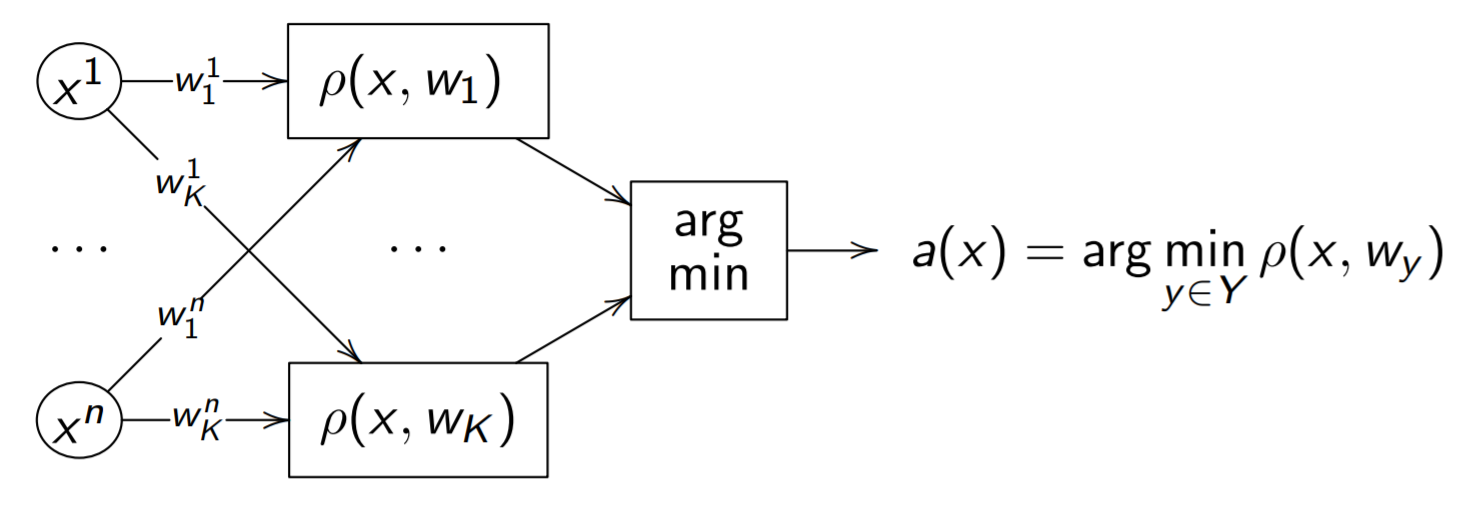
\includegraphics[keepaspectratio,
                      width=0.7\paperwidth]{kohonen-net.png}
   \end{center}

   \pause
   Gradient step in stochastic gradient descent:

   $$w_y = w_y + \eta(x_i-w_y)[a(x_i)=y]$$

   If $x_i$ belongs to the cluster $y$, then $w_y$ is shifted towards $x_i$

   \vspace{0.5cm}
   \noindent\rule{8cm}{0.4pt}

   {\footnotesize 
   {\it T. Kohonen.} Self-organized formation of topologically correct feature maps. 1982.}
\end{frame}


\note{Actually we can write the same operations in the form of special two-layer neural network. And of course you use stochastic gradient descent for optimization of our network. }


\begin{frame}
  \frametitle{Stochastic Gradient Descent}

   {\bf Input}: sample $X^\ell$, learning rate $\eta$, parameter $\lambda$

   {\bf Output}: cluster centers $w_1, \dots, w_K \in \mathbb{R}^n$

   \pause
   \begin{enumerate}
     \item initialize centers $w_y,\ y \in Y$
     \pause
     \item functional estimate: $${Q} = \sum\limits_{i=1}^\ell \rho^2(x_i, w_{a(x_i)}) $$
     \pause
     \item {\bf repeat}
       \begin{itemize}
         \item select object $x_i$ from $X^\ell$ (e.g. random)
         \item compute cluster: $y = \arg\min\limits_{y \in Y} \rho(x_i, w_y)$
         \item make a gradient step: $\color{red}{w_y = w_y + \eta (x_i - w_y)}$
         \item evaluate functional: ${Q} = \lambda \rho^2(x_i, w_y) + (1 - \lambda) {Q}$
       \end{itemize}
     \pause
     \item {\bf while} the value of ${Q}$ and/or the weights of $w_y$ do not converge
   \end{enumerate}
\end{frame}

\note{Ok, here we have written down all the steps of SGD in this case.}

\begin{frame}
\frametitle{Hard and soft competition}

   {\bf WTA, Winner Takes All}

   $$w_y = w_y + \eta(x_i-w_y){\color{red}[a(x_i)=y]}, y \in Y$$

   {\bf WTA rule disadvantages}
   \begin{itemize}
     \item slow convergence rate
     \item some cluster centers may never be selected
   \end{itemize}

   \pause
   {\bf Soft competition rule (WTM, Winner Takes Most)}

   $$w_y = w_y + \eta(x_i-w_y){\color{red}K(\rho\left(x_i, w_y)\right)}, y \in Y$$

   where the kernel $K(\rho)$ is a nonnegative non-increasing function.

   Now the centers of all clusters are shifted towards $x_i$, but the farther from $x_i$, the smaller the shift
\end{frame}

\note{Now let's compare two rules of competition. The first one is the Winner Takes All rule, we used it on previous slides. The second one is a little bit softer, the Winner Takes Most rule.}

\begin{frame}
  \frametitle{Kohonen Map (Self Organizing Map, SOM)}

   We introduce a rectangular grid of clusters $\{1, \dots, SizeX\}\times \{1, \dots, SizeY\}$

   Each node $(x, y)$ is assigned a Kohonen neuron $w_{xy} \in \mathbb{R}^n$

   Along with the metric $\rho(x_i, w_{xy})$, a metric on the grid is introduced:

   $$ r((x, y),(a, b)) = \sqrt{(x - a)^2 + (y - b)^2}$$

   \begin{center}
     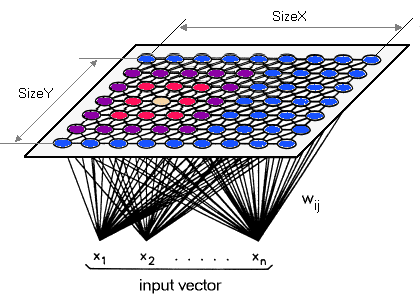
\includegraphics[keepaspectratio,
                      width=0.5\paperwidth]{kohonen-net-scheme.png}
   \end{center}
\end{frame}

\note{Finally, now we can formulate a new unusual approach to the clustering problem, which is called Kohonen Map (or Self Organizing Map). So we introduce a rectangular grid of clusters, where each node (x, y) is assigned to a Kohonen neuron $w_xy \in R^n$.}

\begin{frame}
  \frametitle{Kohonen Map Training}

   {\bf Input}: sample $X^\ell$, learning rate $\eta$

   {\bf Output}: $w_{xy} \in \mathbb{R}^n$ are weight vectors

   \pause
   \begin{enumerate}
     \item initialize weights: $w_{xy} = \text{random}\left(-\frac{1}{2MH}, \frac{1}{2MH} \right)$
     \pause
     \item {\bf repeat}
     \begin{itemize}
       \item choose a random object $x_i$ from $X^\ell$
       \item WTA: compute cluster coordinates: $$(a_i, b_i) = \arg\min\limits_{(a, b)} \rho(x_i, w_{ab})$$
       \item {\bf for all} $(a, b) \in $ Neighborhood $(a_i, b_i)$

        $\ \ \ $ WTM: do gradient descent step:

        $\ \ \ $ $w_{ab} = w_{ab} + \eta (x_i - w_{ab}) K(r((a_i, b_i), (a, b)))$
     \end{itemize}
     \pause
     \item {\bf yet} clustering does not stabilize
   \end{enumerate}
\end{frame}

\note{How do we train it?}


\begin{frame}
  \frametitle{Interpretation of Kohonen Maps}

    Two types of graphs — color maps $SizeX \times SizeY$

   \begin{itemize}
     \item Node color $(a, b)$ — local density at point $(a, b)$ — average distance to $k$ closest sample points
     \item One card for each feature: node color $(a, b)$ — value of $j$-th component of vector $w_{ab}$
   \end{itemize}
   \pause
   \vspace{1cm}
   \begin{exampleblock}{Example}
   Let's look at Kohonen's maps, built on six features collected from 1000 people.
   \end{exampleblock}
\end{frame}

{ % all template changes are local to this group.
    \setbeamertemplate{navigation symbols}{}
    \begin{frame}<article:0>[plain]
        \begin{tikzpicture}[remember picture,overlay]
            \node[at=(current page.center)] {
                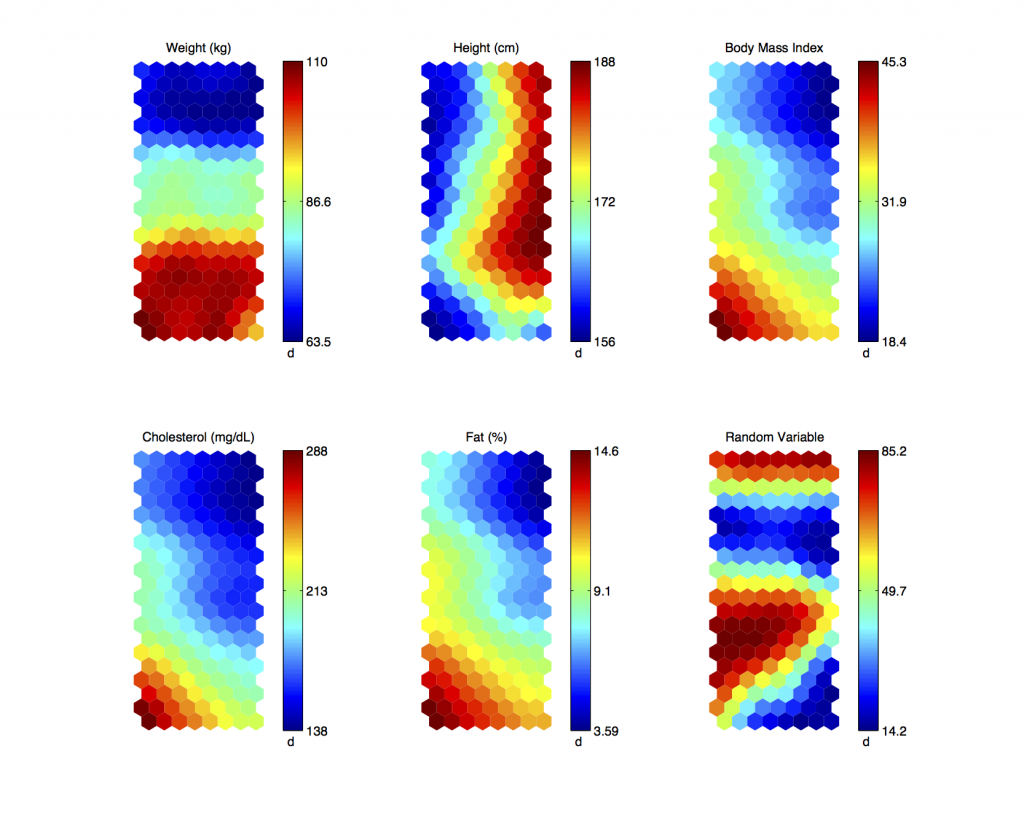
\includegraphics[keepaspectratio,
                                 width=\paperwidth,
                                 height=\paperheight]{kohonen-map.png}
            };
        \end{tikzpicture}
     \end{frame}
}


\begin{frame}[t]
\frametitle{Pros and cons of Kohonen cards}

    $+$ visual analysis of multidimensional data

    $-$ {\bf Distortion}. Close objects in the original space can move to far points on the map, and vice versa

    $-$ {\bf Subjectivity}. The map depends not only on the cluster data structure, but also on...

    \begin{itemize}
      \item properties of the smoothing kernel
      \item (random) initialization
      \item of (random) selection of $x_i$ during iterations
    \end{itemize}

    \pause
    \vspace{1cm}
    Well suited for exploratory data analysis (EDA).
\end{frame}


\begin{frame}
  \frametitle{Autoencoders}

    \begin{center}
      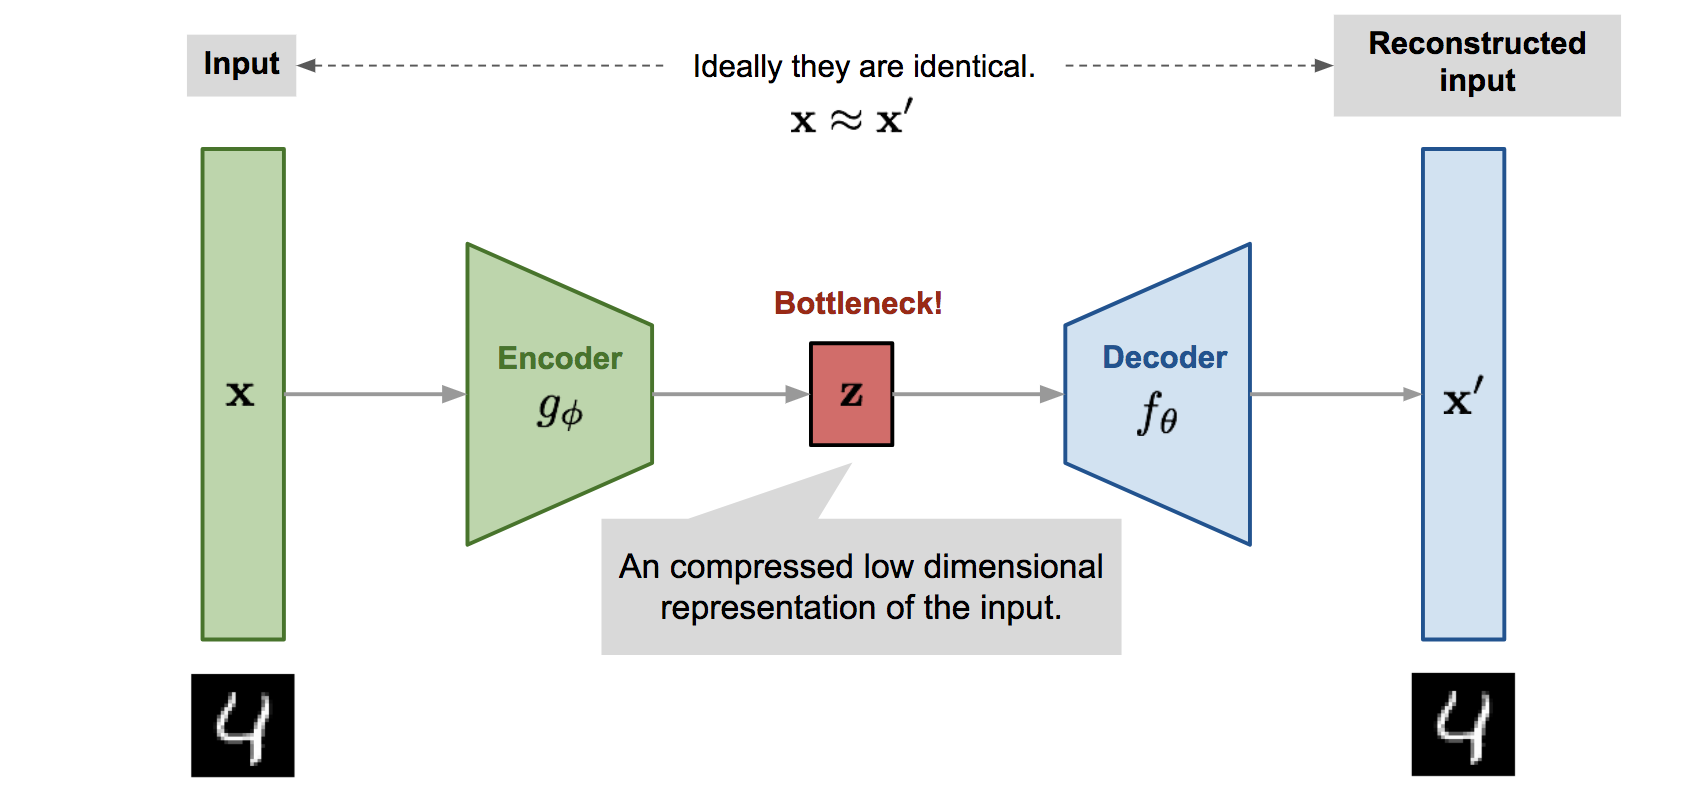
\includegraphics[keepaspectratio,
                       width=0.9\paperwidth]{autoencoder-architecture.png}
    \end{center}
    
    \pause
    \begin{block}{Question}
      What can be used as encoder and decoder here?
    \end{block}
\end{frame}

\note{Ok, great. Now let's move on to another interesting approach in machine learning. It is autoencoders and it's main idea is quite simple. So you have some input vector, for example an image. Then you have two parts of the model, which are the encoder part, where you get some representation of the input, and the decoder part, where you try to get back to the initial input vector.}


\begin{frame}
  \frametitle{Ways to use autoencoders}
    \begin{itemize}
      \item Feature generation, for example, to effectively solve supervised learning problems
      \item Dimensionality reduction
      \item Low loss data compression
      \item Trainable object vectorization, embeddable in deeper neural network architectures
      \item Generation of synthetic objects similar to real ones
    \end{itemize}

  \vspace{1cm}
  \noindent\rule{8cm}{0.4pt}

  {\footnotesize
  {\it Rumelhart, Hinton, Williams}. Learning Internal Representations by Error Propagation. 1986.

  {\it David Charte et al}. A practical tutorial on autoencoders for nonlinear feature fusion: taxonomy, models, software and guidelines. 2018.}
\end{frame}


\begin{frame}
  \frametitle{Linear auto encoder and principal component analysis}

    $$ \mathscr{L}_{AE}(A, B) = \sum\limits_{i = 1}^\ell \|{\color{red}BA}x_i - x_i \|^2 \to \min \limits_{A,B}$$

    Principal Component Analysis: $F = (x_1\dots x_\ell)^T, U^TU = I_m, G = FU,$

    $$\|F - GU^T \|^2 = \sum\limits_{i = 1}^\ell \|{\color{red}UU^T}x_i - x_i \|^2 \to \min\limits_{U}$$

    \pause
    The autoencoder generalizes the principal component analysis:
    \begin{itemize}
      \pause
      \item it is not necessarily $B=A^T$ (although this is often done)
      \pause
      \item arbitrary $A, B$ instead of orthogonal
      \pause
      \item non-linear models
      \pause
      \item arbitrary loss function $\mathscr{L}$ instead of quadratic
      \pause
      \item SGD optimization instead of singular value decomposition (SVD)
    \end{itemize}
\end{frame}


\begin{frame}
  \frametitle{Sparse auto encoder}

    \begin{exampleblock}{Reminder from SVM}
    If the loss function has a kink, then we select objects. If regularizer has a kink, then we select features.
    \end{exampleblock}

   \begin{itemize}
     \item Applying $L_1$ or $L_2$ regularization to weight vectors
     \item Applying of $L_1$-regularization to representation vectors $z_i = Ax_i$
     \item Entropy regularization
   \end{itemize}

   \vspace{1cm}
   \noindent\rule{8cm}{0.4pt}

   {\footnotesize
   {\it D.Arpit et al}. Why regularized auto-encoders learn sparse representation? 2015}
\end{frame}


\begin{frame}
  \begin{center}
    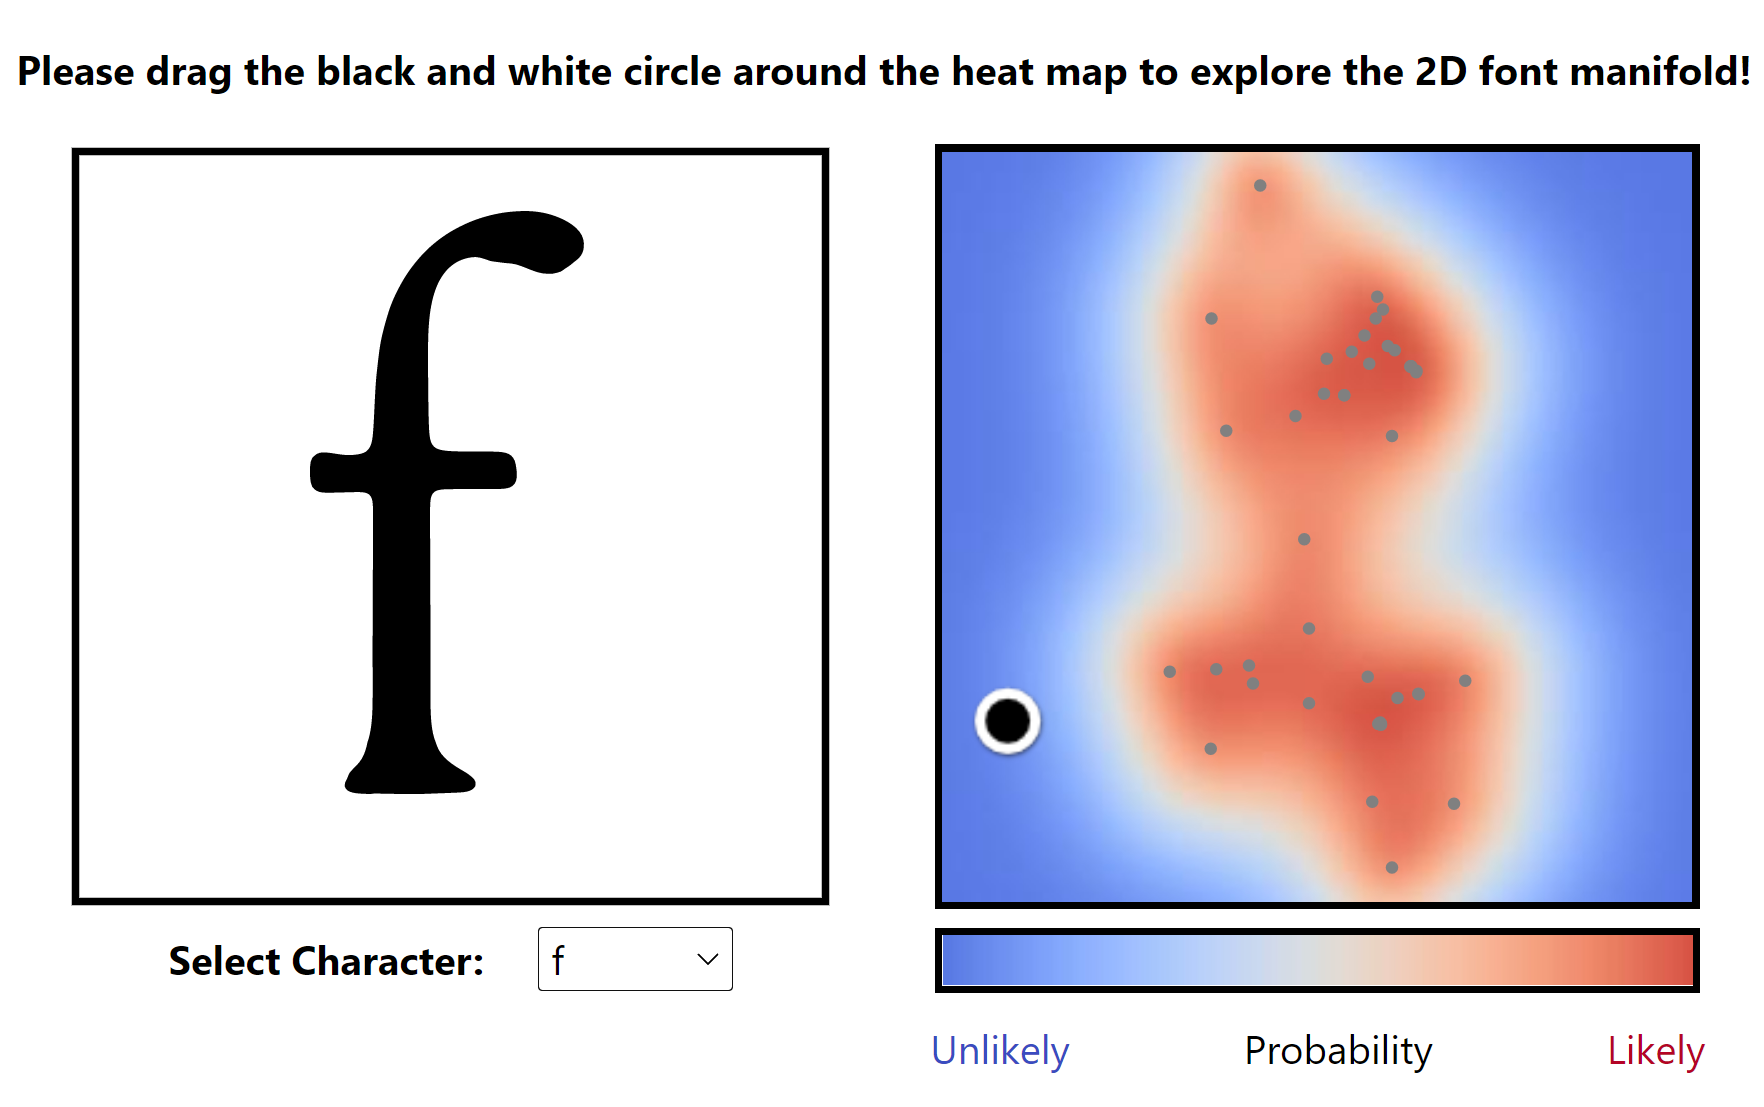
\includegraphics[keepaspectratio,
                     width=0.8\paperwidth]{2d-font-manifold.png}

  \href{https://www.ndfcampbell.org/research/fonts/}{2d font manifold demonstration}
  \end{center}
\end{frame}

\note{Here let's enjoy a little demo where different fonts are nested in a 2D plane.}

\begin{frame}
  \frametitle{Denoising Auto Encoder}

  Stability of code vectors $z_i$ with respect to noise in $x_i$:

  $$\mathscr{L}_{DAE}(\alpha, \beta) = \sum\limits_{i = 1}^\ell {\color{red} E_{\tilde x \sim q(\tilde x| x_i)}}
  \mathscr{L}(g(f({\color{red}\tilde x}, \alpha), \beta),x_i) \to \min\limits_{\alpha, \beta}$$

  \begin{columns}
      \begin{column}{.6\paperwidth}
        Instead of calculating the expectation $E_{\tilde x}$ in the stochastic gradient method, $x_i$ objects are sampled and noisy one at a time: $\tilde x \sim q(\tilde x|x_i)$
        \begin{itemize}
          \item Gaussian noise: $\tilde x \sim N(x_i, \sigma^2 I)$
          \item zeroing components of vector $x_i$ with probability $p_0$
        \end{itemize}
      \end{column}
      \begin{column}{.3\paperwidth}
        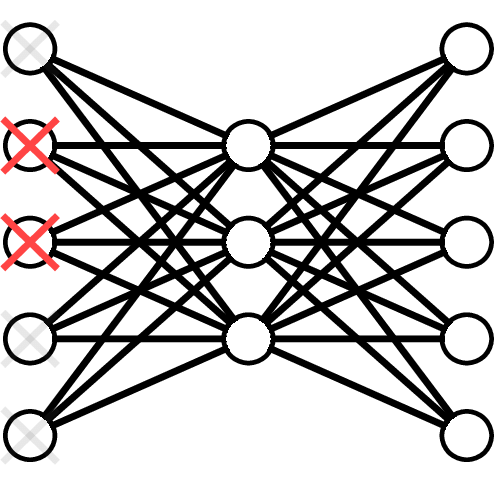
\includegraphics[keepaspectratio,
                       width=.3\paperwidth]{denoising-AE.png}
      \end{column}
  \end{columns}

  \noindent\rule{8cm}{0.4pt}

  {\footnotesize
  {\it P. Vincent, H. Larochelle, Y. Bengio, P.-A. Manzagol}. Extracting and composing robust features with denoising autoencoders. ICML-2008.}
\end{frame}

\note{Ok, now let's discuss briefly a few more autoencoders. For a example, the denoising one.}

\begin{frame}
  \frametitle{Variational Auto Encoder}

  A generative model is constructed capable of generating new objects $x$ similar to the objects of the sample $X^\ell = \{x_1,\dots,x_\ell \}$

   $q_\alpha(z|x)$ — probabilistic encoder with $\alpha$ parameter

   $p_\beta(\hat x|z)$ — probabilistic decoder with $\beta$ parameter

    \begin{align*}
    \mathscr{L}_{VAE}(\alpha, \beta) = \sum\limits_{i=1}^\ell \log p(x_i) = \sum\limits_{i=1}^\ell \log \int q_{\alpha} (z | x_i) \frac{p_{\beta}(x_i|z) p(z)}{q_{\alpha} (z | x_i)} dz \geq \\
     \geq \sum\limits_{i=1}^\ell \int q_\alpha(z|x_i) \log p_\beta(x_i|z)dz - KL(q_\alpha(z|x_i)\| p( z)) \to \max\limits_{\alpha, \beta}
    \end{align*}

  \vspace{0.5cm}
  \noindent\rule{8cm}{0.4pt}

  {\footnotesize
  {\it D.P.Kingma, M.Welling.} Auto-encoding Variational Bayes. 2013.

  {\it C.Doersch.} Tutorial on variational autoencoders. 2016.}
\end{frame}


\note{The next one is Variational Auto Encoder and it may be difficult to understand from the first view, but it's main feature is to use lower variational bound of log likelihood of your model.}


\begin{frame}

$$\sum\limits_{i=1}^\ell \underbrace{E_{z \sim q_{\alpha}(z|x_i)} \log p_\beta(x_i|z)}_{\text{quality reconstruction}} -
\underbrace{KL(q_\alpha(z|x_i)\| p(z))}_{
   \text{regularizer by } \alpha
}
\to \max\limits_{\alpha, \beta}$$

where $p(z)$ is the prior distribution, usually $N(0, \sigma^2 I)$

\pause
\vspace{1cm}
{\bf Reparametrization} $q_\alpha (z|x_i):\ z = f(x_i, \alpha, \varepsilon),\ \varepsilon \sim N(0, I)$

\pause
\vspace{0.5cm}{\bf Stochastic gradient method}:
\begin{itemize}
   \item sample $x_i \sim X^\ell,\ \varepsilon \sim N(0, I),\ z = f(x_i, \alpha, \varepsilon)$
   \item gradient step
   $ \alpha = \alpha + h \nabla_\alpha[\log p_\beta(x_i|f(x_i, \alpha, \varepsilon)) - KL(q_\alpha(z|x_i)\| p(z)) ] $

   $ \beta = \beta + h \nabla_\beta[\log p_\beta(x_i|z)] $

\end{itemize}

\pause
\vspace{0.5cm}
{\bf Generation of similar objects}: $$x \sim p_\beta(x|f({\color{red}x_i}, \alpha, \varepsilon)), \varepsilon \sim N(0, I)$$
\end{frame}

\note{So we two parts of functional, and first one if responsible for quality reconstruction, second one is actually regularizer by $\alpha$.

To evaluate the expactation of some function with z distribution you need to use reparametrization trick. What is it?
On the first step you sample z-value as value of new function f with new parameter $\epsilon$, which comes from some random distribution, for example normal.
And then on the second step you get the expectation with your z-value.}

\begin{frame}
  \frametitle{Autoencoders for supervised learning}

    {\bf Data:} unlabeled $(x_i)_{i=1}^\ell$, labeled $(x_i, y_i)_{i=\ell+1}^{\ell + k}$
    \begin{align*}
      z_i &= f(x_i, {\color{blue}\alpha}) \text{ — encoder} \\
      \hat x_i &= g(z_i, {\color{green}\beta}) \text{ — decoder} \\
      \hat y_i &= \hat y(z_i, {\color{orange}\gamma}) \text{ — classifier}
    \end{align*}
    \begin{center}
      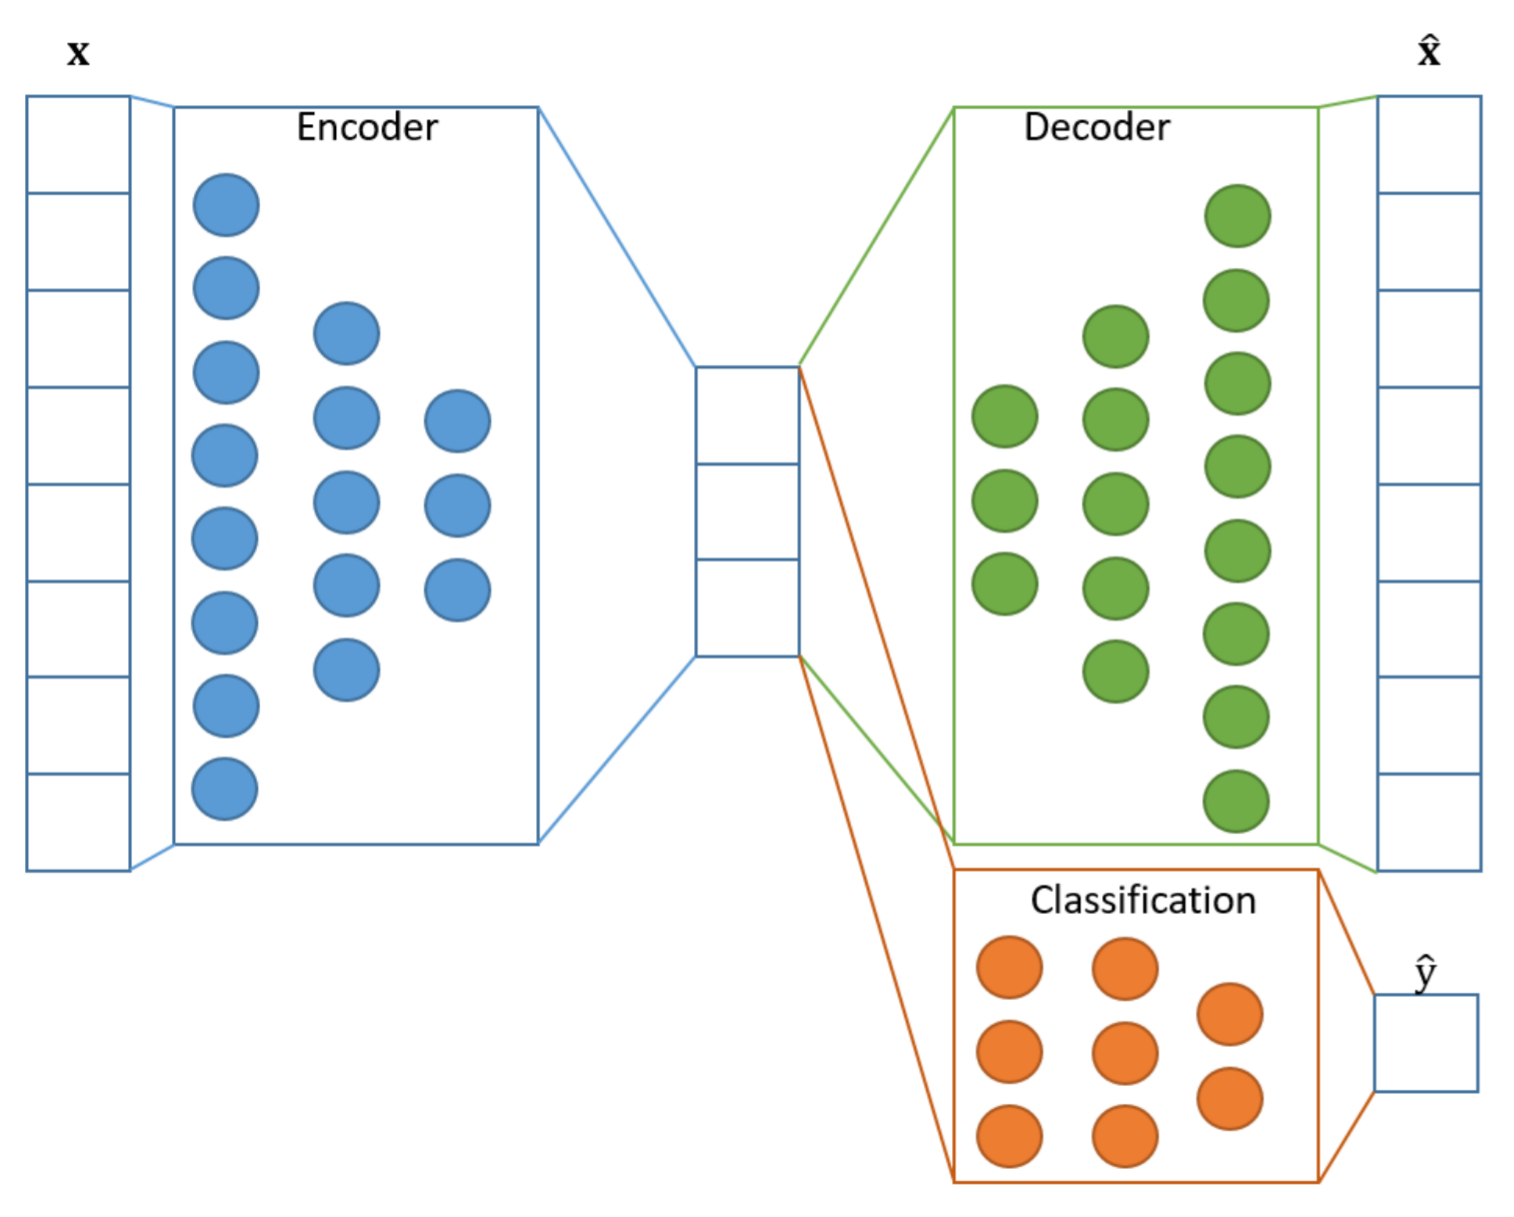
\includegraphics[keepaspectratio,
                       width=.5\paperwidth]{autoenc_supervised.png}
    \end{center}
\end{frame}


\begin{frame}

    {\bf Co-learning} encoder, decoder and predictive model (classification, regression, etc.)

    $$\sum\limits_{i=1}^\ell \mathscr{L}(g(f(x_i, \alpha), \beta), x_i)
    + \lambda \sum\limits_{i=\ell+1}^{\ell+k} \tilde{\mathscr{L}}(\hat y(f(x_i, \alpha), \gamma), y_i) \to \min\limits_{\alpha, \beta, \gamma}$$

    \vspace{0.5cm}
    {\bf Loss functions:}

    $\mathscr{L}(\hat x_i, x_i)$ — reconstruction

    $\tilde{\mathscr{L}}(\hat y_i, y_i)$ — prediction

    \vspace{1cm}

    \noindent\rule{8cm}{0.4pt}

    {\footnotesize
    {\it Dor Bank, Noam Koenigstein, Raja Giryes.} Autoencoders. 2020.}
\end{frame}


\begin{frame}
  \frametitle{Pre-training of neural networks}

    Convolutional network for image processing:

    \begin{itemize}
      \item $\color{red}{z=f(x,\alpha)}$ — convolutional layers for object vectorization
      \item $y = g(z, \beta)$ — fully connected layers for a specific problem
    \end{itemize}

    \begin{center}
      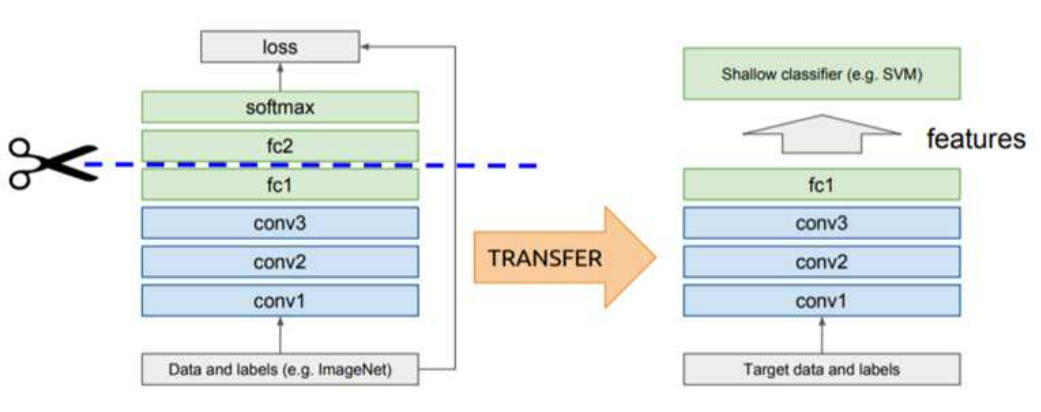
\includegraphics[keepaspectratio,
                       width=.8\paperwidth]{pre-training.png}
    \end{center}

    \noindent\rule{8cm}{0.4pt}

    {\footnotesize
    {\it Jason Yosinski, Jeff Clune, Yoshua Bengio, Hod Lipson.} How transferable are features in deep neural networks? 2014.}
\end{frame}


\begin{frame}
  \frametitle{Transfer learning}

    \begin{itemize}
      \item ${\color{red}f(x,\alpha)}$ — universal part of the model (vectorization)
      \item $g(x, \beta)$ — task-specific part of the model
    \end{itemize}

    {\it Basic problem} on sample $\{x_i\}_{i=1}^\ell$ with loss function $\mathscr{L}_i$:

    $$\sum\limits_{i=1}^\ell \mathscr{L}_i ({\color{red}f(x_i,\alpha)}, g(x_i, \beta)) \to \min_{\alpha,\beta} $$

    {\it Target problem} on another sample $\{x_i^\prime\}_{i=1}^m$ with other $\mathscr{L}_i^\prime, g^\prime$:

    $$\sum\limits_{i=1}^m \mathscr{L}_i^\prime ({\color{red}f(x_i^\prime,\alpha)}, g^\prime(x_i^\prime , \beta^\prime)) \to \min_{ \beta^\prime} $$

    with $m \ll \ell$ this can be much better than

    $$\sum\limits_{i=1}^m \mathscr{L}_i^\prime (f(x_i^\prime,\alpha), g^\prime(x_i^\prime, \beta^\prime) ) \to \min_{\alpha, \beta^\prime} $$

    \noindent\rule{8cm}{0.4pt}

    {\footnotesize
    {\it Sinno Jialin Pan, Qiang Yang.} A Survey on Transfer Learning. 2009}
\end{frame}


\begin{frame}
  \frametitle{Multi-task learning}

  \begin{itemize}
    \item ${\color{red}f(x,\alpha)}$ — universal part of the model (vectorization)
    \item $g(x, \beta)$ — specific parts of the model for problems $t \in T$
  \end{itemize}

  Simultaneous training of the model $f$ on tasks $X_t, t \in T$:

  \begin{center}
    $\sum\limits_{t \in T} \sum\limits_{i \in X_t} \mathscr{L}_{ti} ({\color{red}f(x_{ti},\alpha)}, g (x_{ti}, \beta_t)) \to \min_{\alpha, \{\beta_t\}}$
  \end{center}

  \pause
  \vspace{0.2cm}
  {\it Learnability}: the quality of solving a particular problem $\left< X_t, \mathscr{L}_t, g_t\right>$
  improves with increasing sample size $\ell_t = |X_T|$.

  \pause
  \vspace{0.2cm}
  {\it Learning to learn}: the quality of the solution of each of the problems $t \in T$ improves with the growth of $\ell_t$ and the total number of problems $|T|$.

  \pause
  \vspace{0.2cm}
  {\it Few-shot learning}: a small number of examples, sometimes even one, is enough to solve the $t$ problem.

  \noindent\rule{8cm}{0.4pt}

  {\footnotesize
  {\it M.Crawshaw.} Multi-task learning with deep neural networks: a survey. 2020

  {\it Y.Wang et al.} Generalizing from a few examples: a survey on few-shot learning. 2020}
\end{frame}


\note{The hot topic of the last couple of years is exactly multitask and multi-domain training. So we want to have one AI model, which is good for all tasks =) Something like another one step on the way to general AI.}


\begin{frame}
  \frametitle{Self-supervised learning}

  The vectorization model ${\color{red}z=f(x,\alpha)}$ is trained to predict the relative positions of pairs of fragments of the same image

  \begin{center}
    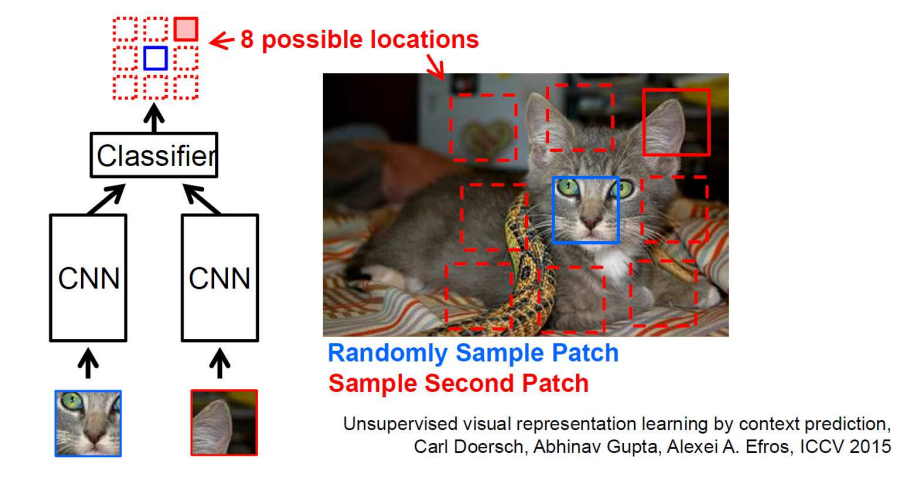
\includegraphics[keepaspectratio,
                     width=.7\paperwidth]{self-supervised.png}
  \end{center}

  {\bf Benefit:} the network learns vector representations of objects without a labeled training set. Their quality is not less than obtained by labeled ImageNet.
\end{frame}


\begin{frame}
  \frametitle{Model distillation or surrogate modeling}

  Training ${\color{red}\text{complex model } a(x, w)}$ is ``long time, expensive'':
  $$\sum\limits_{i=1}^\ell \mathscr{L}({\color{red}a(x_i, w)}, y_i) \to \min_{w}$$
  Training ${\text{simple model } b(x, w^\prime)}$, possibly on other data:
  $$\sum\limits_{i=1}^k \mathscr{L}({b(x_i^\prime, w^\prime)}, {\color{red}a(x_i^\prime, w)} ) \to \min_{w^\prime} $$
  \pause
  {\bf Problem examples:}
  \begin{itemize}
    \item replacement of a complex model (climate, aerodynamics, etc.), which takes months to calculate on a supercomputer, with an ``light'' approximating surrogate model
    \item replacement of a complex neural network, which is trained for weeks on big data, with an ``light'' approximating neural network with minimization of the number of neurons and connections
    \end{itemize}
\end{frame}


\begin{frame}
  \frametitle{Generative Adversarial Net, (GAN)}

  The generator $G(z)$ learns to generate objects $x$ from noise $z$

  The discriminator $D(x)$ learns to distinguish them from real objects

  \begin{center}
    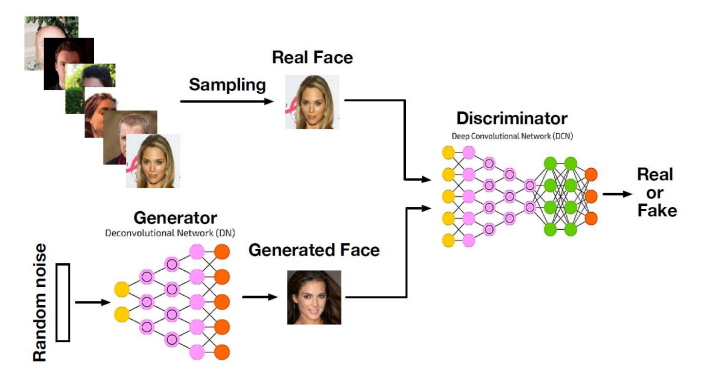
\includegraphics[keepaspectratio,
                     width=.65\paperwidth]{GAN_scheme.png}
  \end{center}

  \noindent\rule{8cm}{0.4pt}

  {\tiny
  {\it Antonia Creswell et al.} Generative Adversarial Networks: an overview. 2017.

  {\it Zhengwei Wang, Qi She, Tomas Ward.} Generative Adversarial Networks: a survey and taxonomy. 2019.

  {\it Chris Nicholson.} \href{https://pathmind.com/wiki/generative-adversarial-network-gan}{A Beginner's Guide to Generative Adversarial Networks}. 2019.
  }
\end{frame}


\begin{frame}
  \frametitle{GAN problem statement}

  There is a selection of objects $\{x_i\}_{i=1}^m$ from $X$

  We train

  \begin{itemize}
    \item probabilistic generative model $G(z, \alpha): x \sim p(x|z,\alpha)$
    \item probabilistic discriminative model $D(x, \beta) = p(1| x, \beta)$
  \end{itemize}

  \pause
   {\bf Criteria}:
   \begin{itemize}
     \item Discriminative model training $D$:
     $$ \sum\limits_{i=1}^m \ln D(x_i, {\color{red}\beta}) + \ln(1 - D(G(z_i, \alpha), {\color{red}\beta})) \to {\color{red}\max\limits_{\beta}}$$
     \item learning the generative model $G$ from random noise $\{z_i\}_{i=1}^m$:
     $$ \sum\limits_{i=1}^m \ln(1 - D(G(z_i, {\color{red}\alpha}), \beta)) \to {\color{red}\min\ limits_{\alpha}}$$
   \end{itemize}

  \noindent\rule{8cm}{0.4pt}

  {\footnotesize
  {\it Ian Goodfellow et al.} Generative Adversarial Nets. 2014}
\end{frame}


\begin{frame}
  \frametitle{StyleGAN demo}

  \href{https://www.youtube.com/watch?v=kSLJriaOumA}{Let's watch the video}

  \vspace{2cm}
  Papers are here: \href{https://nvlabs.github.io/stylegan2/versions.html}{https://nvlabs.github.io/stylegan2/versions.html}

\end{frame}

\begin{frame}
\frametitle{Summary}
   \begin{itemize}
     \item Clustering and Kohonen maps
     \item Autoencoders including co-learning with classification
     \item Multi-task learning
     \item Transfer learning
     \item Distillation and surrogate modeling
     \item Adversarial networks (GANs)
   \end{itemize}
   \pause
   \vspace{0.5cm}
   What else can you see?
   \begin{itemize}
     \item \href{https://www.lektorium.tv/node/36609}{Mini-course by S.I. Nikolenko} about GANs from three lectures (in Russian)
     \item \href{https://www.youtube.com/watch?v=5WoItGTWV54}{Lec. 13} of the CS231n GAN course
   \end{itemize}
\end{frame}

\begin{frame}
  \frametitle{Learning Using Privileged Information (LUPI)}

  \begin{center}
    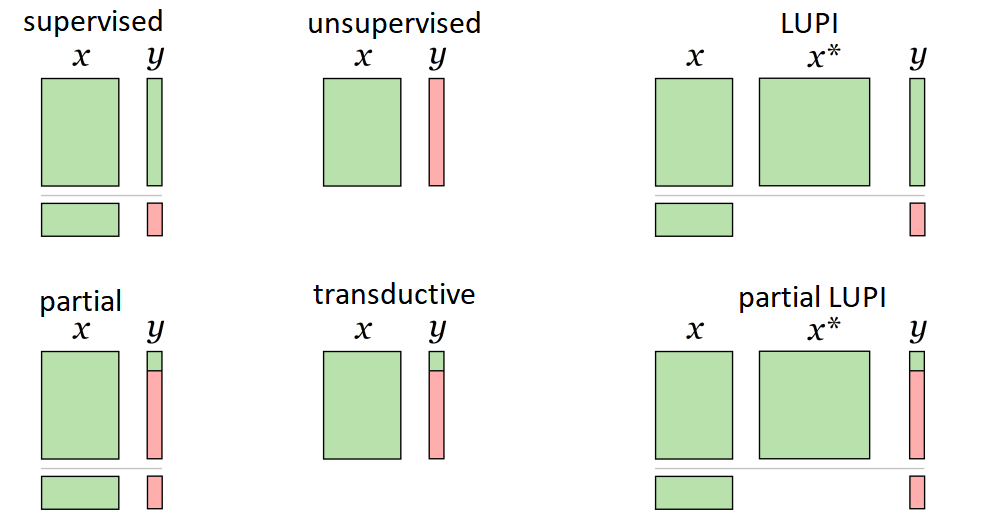
\includegraphics[keepaspectratio,
                     width=.8\paperwidth]{LUPI_en.png}
  \end{center}

  \noindent\rule{8cm}{0.4pt}

  {\footnotesize
  {\it V.Vapnik, A.Vashist.} A new learning paradigm: Learning Using Privileged Information // Neural Networks. 2009.}
\end{frame}


\begin{frame}
\frametitle{Examples of problems with privileged information $x^*$}
  \begin{itemize}
    \item $x$ — primary (1D) protein structure

          $x^*$ — tertiary (3D) protein structure

          $y$ — hierarchical classification of protein function
    \item $x$ — history of the time series

          $x^*$ — information about the future behavior of the series

          $y$ — forecast of the next point of the series
    \item $x$ — text document

          $x^*$ — highlighted keywords or phrases

          $y$ — document category
    \item $x$ — pair (request, document)

          $x^*$ — keywords or phrases highlighted by the assessor

          $y$ — relevance score
  \end{itemize}
\end{frame}


\begin{frame}
  \frametitle{Problem of Learning with Privileged Information}

  \begin{itemize}
    \item Separate training of student model and {\color{red} teacher model}:

    $\sum\limits_{i=1}^\ell \mathscr{L}(a(x_i, w), y_i) \to \min_{w} \quad\quad
    \sum\limits_{i=1}^\ell \mathscr{L}({\color{red}a(x_i^*, w^*)}, y_i) \to \min_{w} $

    \item The student model learns to repeat the mistakes of the {\color{red} teacher model}:

    $\sum\limits_{i=1}^\ell \mathscr{L}(a(x_i, w), y_i) + \mu
     \mathscr{L}(a(x_i, w), {\color{red}a(x_i^*, w^*)}) \to \min_{w} $

    \item {\bf Co-learning} student model and {\color{red} teacher model}:

    \begin{multline*}
    \sum\limits_{i=1}^\ell \mathscr{L}(a(x_i, w), y_i) + \\
    + \lambda \mathscr{L}({\color{red}a(x_i^*, w ^*)}, y_i) 
    + \mu \mathscr{L}(a(x_i, w), {\color{red}a(x_i^*, w^*)}) \to \min_{w, w^*}
    \end{multline*}
  \end{itemize}

  \vspace{0.5cm}
  \noindent\rule{8cm}{0.4pt}

  {\footnotesize
  {\it D.Lopez-Paz, L.Bottou, B.Scholkopf, V.Vapnik.} Unifying distillation and privileged information. 2016.}
\end{frame}

\end{document}
